\section{Question 1 --- River Forecasting Proposal}

\textbf{Proposal in one sentence.} A small, physics-shaped spatio-temporal graph network forecasts the
change in water level at S1--S4 over the next hour as quantiles. It routes upstream information along
the river graph with stage-dependent travel times, feeds announced reservoir releases in as known future
forcing, and adds the predicted change to the last observed level.

\subsection{Architecture diagram}

\begin{figure}[H]
\centering
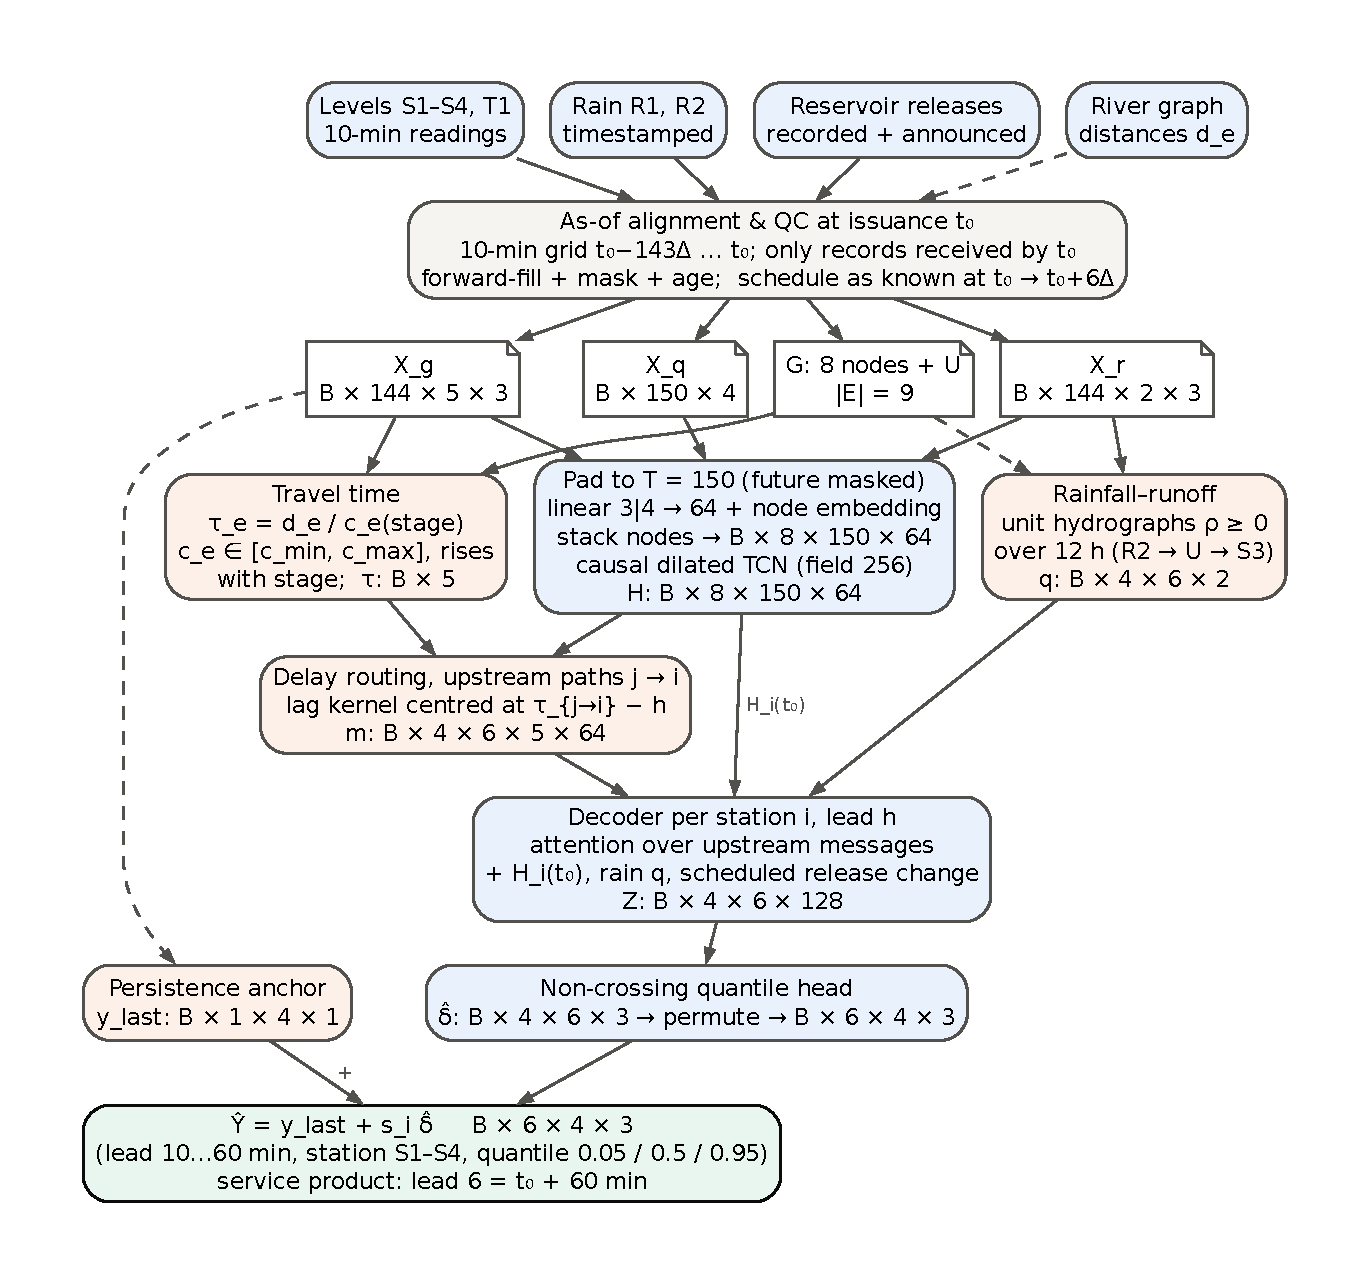
\includegraphics[width=0.93\textwidth]{q1_architecture.pdf}\\[2pt]
\begin{minipage}[c]{0.40\textwidth}
\centering
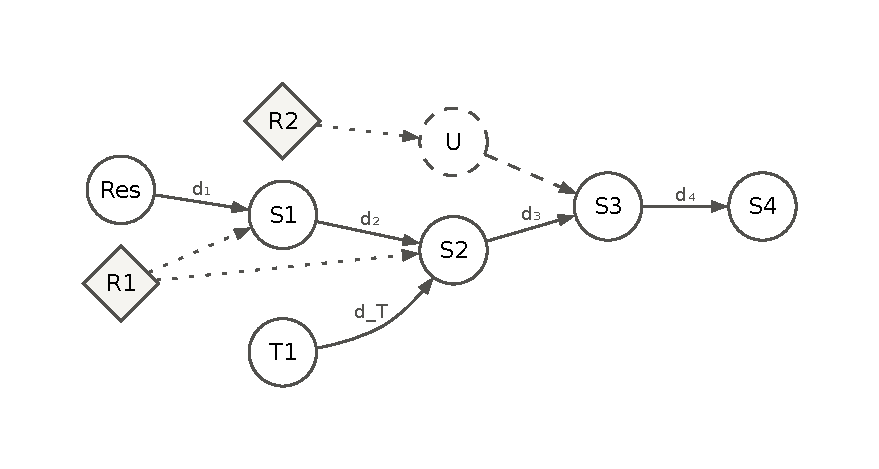
\includegraphics[width=\textwidth]{q1_river_graph.pdf}
\end{minipage}\hfill
\begin{minipage}[c]{0.57\textwidth}
\caption{Architecture (top) and the river graph used for routing (left). Blue blocks are learned networks;
orange blocks have a fixed physical form with a few learned parameters; note-shaped boxes are the input
tensors (axes are listed in the table of Section~\ref{sec:q1-task}). Forecasts are issued at $t_0$, and
$\Delta = 10$\,min. In the graph, solid arrows are channel reaches of length $d_e$, the dashed node $U$ is
the unmonitored tributary (no data; its inflow is inferred), and dotted arrows attach the rain gauges to
the catchments they represent.}
\label{fig:q1-arch}
\end{minipage}
\end{figure}

\subsection{Assumptions}

\textbf{Supplied facts.}
\textbf{F1}: 10-min water levels at S1--S4 and T1.
\textbf{F2}: rainfall at R1 and R2 with timestamps and gauge locations.
\textbf{F3}: recorded releases and schedules announced before issuance, with announcement and effective times.
\textbf{F4}: station locations, connectivity and along-river distances.
\textbf{F5}: travel times and the unmonitored tributary's inflow are not supplied; future rainfall and future
levels are unavailable at issuance.
Everything below is an \emph{assumption}, chosen to be the most defensible reading where the brief is silent.

{\small
\begin{longtable}{@{}p{0.04\textwidth}p{0.33\textwidth}p{0.25\textwidth}p{0.32\textwidth}@{}}
\toprule
ID & Assumption & Why it is reasonable & Effect on the design \\ \midrule
\endhead
A1 & All timestamps use one clock (stored in UTC). Readings are nominally every 10\,min with up to $\pm 2$\,min jitter. & Standard for telemetered gauges. & Every reading is assigned to the grid slot $(t-\Delta, t]$ that contains it (Section~\ref{sec:q1-task}). \\
A2 & Most records arrive within 5\,min, but outages can delay them by hours. Each record keeps its \emph{arrival} time. & Typical of radio/cellular telemetry. & Inputs are assembled \emph{as of} $t_0$ by arrival time, and a data-age feature marks staleness. Training replays arrival times (if they are not logged, see request I5). \\
A3 & At least 3 years of overlapping records exist, with several high-flow events and an archive of schedules \emph{as announced}. & The minimum for learning seasonal and event behaviour. & A small model (about $2\times10^5$ parameters) with physical structure. Train/validation/test split chronologically by year, with flood events in every split. \\
A4 & Level sensors are accurate to $\pm$1--2\,cm, with occasional spikes, flat-lines and logged datum shifts. Rain gauges are tipping buckets (0.2\,mm) that under-catch in wind. & Typical gauge specifications. & Range and rate-of-change checks turn bad values into missing values. The sensor noise sets the floor for useful accuracy. \\
A5 & Between stations, water only flows downstream; backwater at the confluences is negligible. & Steep mountain river (see the illustration). & Directed graph: a station only uses data from upstream nodes. \\
A6 & Travel time depends on the water level: higher water gives a faster flood wave (in-bank kinematic-wave behaviour), with mean velocities between 0.3 and 4\,m/s. & Standard open-channel hydraulics. & Each edge's wave speed $c_e$ is bounded and increases with stage, so its travel time is $d_e/c_e$. \\
A7 & Releases enter just above S1, and a release change reaches S1 within one hour. & S1 is directly below the dam in the map. & Scheduled releases inside the forecast hour act directly on S1, and on downstream stations when their path delay is short. \\
A8 & The unmonitored tributary is driven mainly by rain on its own catchment, which R2 (the nearest gauge) represents best; its baseflow varies slowly. & Gauge proximity in the map; baseflow changes over days. & Pathway R2 $\to U\to$ S3 through a rainfall--runoff kernel. Slow baseflow is absorbed by S3's own history. \\
A9 & R1 represents rain on the hillslopes between the dam and S2. T1 sits upstream of its confluence. & Gauge positions in the map. & R1 connects to every station from S1 down; T1 reaches S2 through edge T1$\to$S2 with its own delay. \\
A10 & Rain affects main-river levels after lags of 30\,min to 12\,h. The total reservoir-to-S4 travel time is under 12\,h. Snowmelt follows a daily cycle. & Small mountain catchment with snow (illustration). & A 24\,h history (144 steps) covers the longest lag and one full daily cycle. The encoder's receptive field is 256 steps. \\
A11 & Gaps can cluster during storms, because power and telemetry fail when flows are high. & Common in flood operations. & Training simulates outages that are concentrated on high-flow periods (Section~\ref{sec:q1-ops}). \\
A12 & Channel geometry, gauge datums and the reservoir's operating policy are stable over the record; slow drift is acceptable. & Needed to learn from history at all. & Periodic retraining plus drift monitoring; out-of-range stages are flagged. \\
\bottomrule
\end{longtable}
}

\subsection{Forecasting task and data specification}
\label{sec:q1-task}

\textbf{Issuance and horizon.} A forecast is issued every 10\,min at grid times $t_0$ (\texttt{hh:m0}), as soon
as the inputs have been assembled, typically within a minute of $t_0$. The \textbf{history window} is $L=144$
steps (24\,h), $t_0-143\Delta,\dots,t_0$, long enough for A10. The model predicts all six leads
$t_0+h\Delta$, $h=1,\dots,6$, jointly. This costs nothing extra, gives the intermediate leads as
supervision, and yields a trajectory for operators. The \textbf{service product} is $h=6$, the level at
$t_0+60$\,min at S1--S4, given as a median and a 90\% interval (quantiles 0.05, 0.5, 0.95).

{\small
\begin{longtable}{@{}p{0.09\textwidth}p{0.14\textwidth}p{0.36\textwidth}p{0.33\textwidth}@{}}
\toprule
Tensor & Shape & Axes and content & Timestamps / time coverage \\ \midrule
\endhead
$X_g$ & $B\times144\times5\times3$ & batch; history step; gauge (S1, S2, S3, S4, T1); [level as a per-station $z$-score, observed mask, data age in hours] & Slots $t_0-143\Delta,\dots,t_0$. Slot $t$ holds the latest reading timed in $(t-\Delta,t]$ that had arrived by $t_0$. \\
$X_r$ & $B\times144\times2\times3$ & batch; history step; rain gauge (R1, R2); [$\log(1+\text{mm})$ summed over the slot, mask, age] & Same slots. Future rain is unknown, so there are no future slots. \\
$X_q$ & $B\times150\times4$ & batch; 144 past + 6 future steps; [recorded release (scaled by capacity), scheduled release as known at $t_0$, recorded-value mask, is-future flag] & $t_0-143\Delta,\dots,t_0+6\Delta$. Past slots hold the actual and the then-scheduled rate; future slots hold the schedule from the latest announcement made by $t_0$. \\
$G$ & 8 data nodes + latent $U$; $|E| = 9$ & directed edges with lengths $d_e$ (km); node types (gauge, rain, reservoir) & Static. \\
$y^{\text{last}}$ & $B\times1\times4\times1$ & batch; --; S1--S4; last valid level in metres & The time of the last valid reading, which is $\le t_0$ (its age is in $X_g$). \\
$\hat Y$ (output) & $B\times6\times4\times3$ & batch; lead $h=1..6$; S1--S4; quantile (0.05, 0.5, 0.95); levels in metres above station datum & $t_0+10,\dots,t_0+60$\,min; served at $h=6$. \\
$Y$, $M_Y$ (training only) & $B\times6\times4$ & observed level at each lead, and a mask for missing targets & $t_0+h\Delta$, $h=1,\dots,6$. \\
\bottomrule
\end{longtable}
}

\textbf{Batch axis.} During training, $B$ is a set of issuance times sampled from the training years
(e.g.\ $B=256$). In operation $B=1$, or $B=2$ when a release scenario is run alongside (Section~\ref{sec:q1-ops}).

\textbf{Alignment across locations and sampling times.} All sources are put on one 10-min grid that ends at $t_0$:
\begin{itemize}
\item \textbf{Levels} snap to their slot (A1). An empty slot is forward-filled from the last valid value, with mask 0, and its age keeps growing.
\item \textbf{Rain} accumulations are summed per slot.
\item \textbf{Releases} are step functions sampled at slot times.
\item \textbf{Schedules} are \emph{as-of joined}: for each future slot, use the rate from the latest announcement whose announcement time is $\le t_0$.
\end{itemize}
Training uses the same rule, so the model never sees a schedule, reading or rain value it would not have had at $t_0$.
Uneven station spacing is not resampled away. It enters through the edge lengths $d_e$ and the travel-time
module, so each station is aligned with the \emph{lagged} state of its upstream nodes, not with their same-time state.
To combine sources in one encoder, gauge and rain inputs are padded with six masked future slots (a common axis, $T=150$),
projected per node type to 64 channels and stacked along the node axis: $B\times8\times150\times64$.

\textbf{Information available at issuance.} Everything that had arrived by $t_0$: levels and rain up to $t_0$,
releases recorded up to $t_0$ (possibly lagging), schedules announced up to $t_0$ (covering the future), and the
static graph. \emph{Not} available: future rain, future levels, schedule changes not yet announced, and the
unmonitored tributary's inflow.

\subsection{Model computations and design justification}

\textbf{Notation.} $\Delta=10$\,min, issuance time $t_0$, lead $h\in\{1,\dots,6\}$, hidden width $d=64$.
Nodes: reservoir $Q$, gauges $S_1$--$S_4$ and $T_1$, rain gauges $R_1$, $R_2$, and latent $U$ (no data).
$\mathrm{Up}(i)$ is the set of gauges and reservoir upstream of station $i$; the graph is a tree, so the path
$j\to i$ is unique. $\sigma$ is the logistic function, and $\mathrm{sp}$ is softplus.

\textbf{(1) Projection and encoder.} For node $j$ of type $\kappa(j)$ and slot $t$:
$e_j(t)=W^{\kappa(j)}x_j(t)+p_j$, where $p_j$ is a learned node embedding. Then 8 residual causal
dilated convolution layers (kernel 2, dilation $2^\ell$) are applied:
\[
H^{(\ell+1)}_j(t)=H^{(\ell)}_j(t)+\mathrm{GELU}\big(W^{(\ell)}_0H^{(\ell)}_j(t)+W^{(\ell)}_1H^{(\ell)}_j(t-2^\ell\Delta)\big),\qquad H_j=H^{(8)}_j\in\mathbb R^{150\times d}.
\]
Causality means $H_j(t)$ only depends on inputs at slots $\le t$. In the future slots, the reservoir carries the
announced schedule, and gauges and rain carry only ``unobserved'' tokens.

\textbf{(2) Travel time (physical form, learned parameters).} For edge $e=(j\to k)$, with $\bar y_j$ and $s_j$ the
training mean and standard deviation of station $j$'s level:
\[
c_e = c^{\min}_e+(c^{\max}_e-c^{\min}_e)\,\sigma\!\big(\mathrm{sp}(\alpha_e)\,(y^{\text{last}}_j-\bar y_j)/s_j+\beta_e\big),\qquad
\tau_e=\frac{d_e}{c_e\,\Delta},\qquad \tau_{j\to i}=\sum_{e\in \mathrm{path}(j,i)}\tau_e .
\]
$c_e$ is bounded (A6) and increases with stage, because $\mathrm{sp}(\cdot)\ge0$. The travel times $\tau$ are
measured in steps and can be read off for checking against hydrological knowledge.

\textbf{(3) Delay routing.} Upstream water that reaches station $i$ at $t_0+h\Delta$ passed node $j$ about
$\tau_{j\to i}$ steps earlier, i.e.\ $k^\star=\tau_{j\to i}-h$ steps before $t_0$. Let $k\in\{-6,\dots,143\}$
count steps before $t_0$ (negative values are future slots). Then:
\[
\kappa_{ji,h}(k)=\frac{\exp\!\big(-(k-k^\star)^2/2\varsigma_{ji}^2\big)}{\sum_{k'}\exp\!\big(-(k'-k^\star)^2/2\varsigma_{ji}^2\big)},\qquad
m_{ji,h}=\sum_k\kappa_{ji,h}(k)\,H_j(t_0-k\Delta),\qquad \phi_{ji,h}=\sum_{k<0}\kappa_{ji,h}(k).
\]
$\varsigma_{ji}=\mathrm{sp}(\cdot)$ is a learned spread that represents wave dispersion (Muskingum-like attenuation).
$\phi_{ji,h}$ is the share of the kernel that falls in the future. For the reservoir, those slots hold the
\emph{announced schedule}, so a release change reaches each station after its physical delay. For a gauge they
hold no data, so $\phi$ tells the decoder that this upstream signal has not arrived yet; the decoder then leans
on nodes further upstream, whose delays are longer.

\textbf{(4) Rainfall--runoff.} Each rain gauge $r$ connects to every station downstream of where it attaches
(R1: S1--S4; R2, through $U$: S3, S4), using a non-negative 12\,h unit hydrograph:
\[
q_{ri,h}=\sum_{\ell=0}^{71}\rho_{ri}(\ell)\,R_r\big(t_0+h\Delta-\ell\Delta\big),\qquad \rho_{ri}(\ell)=\mathrm{sp}(\theta_{ri\ell})\ge0,\qquad R_r(t>t_0)=0 .
\]

\textbf{(5) Decoder and forecast mapping.} Query $u_{i,h}=W_q[H_i(t_0);p_i;\eta_h]$, where $\eta_h$ is a lead
embedding. Each upstream source contributes the key $k_{ji,h}=W_k[m_{ji,h};\tau_{j\to i};\phi_{ji,h}]$:
\[
a_{ji,h}=\operatorname*{softmax}_{j\in\mathrm{Up}(i)}\!\big(u_{i,h}^{\top}k_{ji,h}/\sqrt d\big),\qquad
z_{i,h}=\mathrm{MLP}\big([u_{i,h};\textstyle\sum_j a_{ji,h}W_vk_{ji,h};q_{\cdot i,h};\delta^{Q}_h]\big)\in\mathbb R^{128},
\]
where $\delta^Q_h$ is the scheduled change in release between $t_0$ and $t_0+h\Delta$. The head
$(o_1,o_2,o_3)=W_oz_{i,h}$ gives quantiles of the standardised change that cannot cross:
\[
\hat\delta^{0.5}=o_1,\quad \hat\delta^{0.05}=o_1-\mathrm{sp}(o_2),\quad \hat\delta^{0.95}=o_1+\mathrm{sp}(o_3),\qquad
\hat Y^{(q)}_{h,i}=y^{\text{last}}_i+s_i\,\hat\delta^{q}_{i,h}.
\]

\textbf{(6) Training objective.} A masked pinball loss, weighted towards the service lead ($w_6=2$, $w_{1..5}=1$),
plus a smoothness penalty on the unit hydrographs:
\[
\mathcal L=\frac{\sum_{b,h,i}M_{Y,bhi}\,w_h\sum_{q}\rho_q\big(Y_{bhi}-\hat Y^{(q)}_{bhi}\big)}{\sum_{b,h,i}M_{Y,bhi}\,w_h}
+\lambda\sum_{r,i,\ell}\big(\rho_{ri}(\ell{+}1)-2\rho_{ri}(\ell)+\rho_{ri}(\ell{-}1)\big)^2,\qquad
\rho_q(u)=\max(qu,(q-1)u).
\]
Training uses AdamW with early stopping on the validation pinball loss at $h=6$, and random input masking
(Section~\ref{sec:q1-ops}). Interval widths are then calibrated per station on the validation years
(split-conformal adjustment), so the 90\% band covers about 90\%.

\textbf{Why these choices.}
\begin{itemize}
\item \emph{Predict the change, anchored on the last level.} Over one hour, persistence is the strongest simple
forecast. Learning the change removes datum differences between stations and leaves the network the dynamics.
\item \emph{Explicit travel-time routing instead of stacked message passing.} With $K$ message-passing layers,
information only travels $K$ hops, and it must also arrive at the right \emph{lag}. On a 4-hop chain, routing
along each upstream path gives full reach in hops and in time in one step, with a handful of parameters per
edge. Travel times that change with conditions (A6) are modelled directly instead of being averaged away.
\item \emph{Causal dilated convolutions instead of temporal attention.} A 256-step receptive field costs linear
time and memory. Attention would cost $O(L^2)$, and its main benefit, finding the relevant lag, is already
provided by the routing kernel.
\item \emph{Non-negative unit hydrographs.} More rain can never lower the forecast, and a linear kernel can be
learned from few storms.
\item \emph{Quantile outputs.} Flood preparedness needs risk, e.g.\ $P(\text{S4}>\text{threshold})$, not just a
point value.
\end{itemize}

\textbf{How each driver reaches each forecast.}
\begin{itemize}
\item \textbf{S1}: its own history; the reservoir's recorded and announced releases, with a short delay
(announced changes within the hour matter most); rain at R1.
\item \textbf{S2}: adds S1 and T1, each through its own delay; the reservoir through the path
$Q\to$ S1 $\to$ S2; R1.
\item \textbf{S3}: adds S2 and everything upstream of it. The \emph{unmonitored tributary} enters in two ways:
R2's rainfall--runoff kernel, and S3's own history, whose departure from routed S2 is a running proxy for the
tributary's inflow.
\item \textbf{S4} (next to the town): all of the above through S3 and the longer paths. For short leads, S3's
recent state dominates.
\end{itemize}

\textbf{Physical assumptions versus learned mappings.}
\begin{itemize}
\item \emph{Physical, fixed by design:} graph topology and flow direction, edge lengths, travel time
$=$ distance / wave speed, wave-speed bounds that increase with stage, causal and as-of masking,
non-negative rain response, the persistence anchor, and announced releases entering only through path delays.
\item \emph{Learned:} the wave-speed curves, dispersion, unit hydrographs, encoder, attention, decoder and quantiles.
\end{itemize}
A separate hydraulic simulator is not needed: the physics enters through structure and constraints. A simulator's
output could later be added as one more input node (request I2).

\subsection{Operation and exceptional conditions}
\label{sec:q1-ops}

\textbf{(i) Missing observations.}
\begin{itemize}
\item Missing or quality-rejected values are forward-filled with mask 0 and a growing age, never set to zero, so
input scales stay meaningful.
\item If a station's own reading at $t_0$ is missing, $y^{\text{last}}$ is its last valid value, and the age
feature lets the network widen its intervals and rely on upstream nodes.
\item During training, inputs are randomly masked: single slots, runs of up to 6\,h, and whole-station outages
concentrated on high-flow periods (A11). Missing targets are excluded through $M_Y$.
\item A station whose data are older than 6\,h is flagged ``degraded'' on the dashboard. Its forecast is still
issued, from upstream routing plus its last value.
\end{itemize}

\textbf{(ii) Delayed observations.}
\begin{itemize}
\item Inputs are assembled by \emph{arrival} time (A2). A late reading is invisible to the forecasts issued
before it arrives, and is used automatically from the next issuance on.
\item The model keeps no state between runs (each forecast is recomputed from the 24\,h window), so late data
never corrupt a carried-over state.
\item Training replays the logged arrival times, so the network sees the same kind of staleness it meets in
operation.
\end{itemize}

\textbf{(iii) Announced future releases.}
\begin{itemize}
\item These are \emph{known future inputs}. Each forecast uses the latest announcement made by $t_0$, as-of
joined onto the future slots of $X_q$, and they act through the routing delays ($\phi>0$ for the reservoir).
\item If no announcement covers the hour, the current rate is assumed to continue, and a flag is set.
\item Announcements made \emph{after} $t_0$ are never used, either in training or in operation.
\end{itemize}

\textbf{(iv) Differences between scheduled and actual releases.}
\begin{itemize}
\item Past slots of $X_q$ hold both the recorded and the then-scheduled rate. The network therefore learns how
reliably schedules are followed, and widens its intervals when recent deviations are large.
\item Once a deviation is recorded, it replaces the schedule for those past slots at the next issuance.
\item For operators, a second scenario is run in the same batch ($B=2$: ``as scheduled'' and ``current rate
continues''). The spread between the two shows how sensitive each station is to the release decision.
\end{itemize}

\textbf{Feasibility every 10 minutes.} The model has about $2\times10^5$ parameters. One forecast is a single
forward pass over $8\times150$ node-steps, on the order of $10^7$ multiply-adds: milliseconds on one CPU core.
Assembling 24\,h of records is a few small database queries. A run therefore takes seconds, far inside the
10-minute cycle, which leaves room for scenario runs, an ensemble of seeds and retries. If the model service
fails, persistence plus routed upstream change is issued as a fallback and labelled as such.

\subsection{Uncertainty, limitations, and additional information}

{\small
\begin{longtable}{@{}p{0.2\textwidth}p{0.36\textwidth}p{0.38\textwidth}@{}}
\toprule
Item & Forecast impact & Response, or what remains unresolved \\ \midrule
\endhead
Unmonitored tributary & Its inflow is invisible. This mainly affects S3 and S4 during local storms on its catchment. & Inferred from R2's kernel and S3's departure from routed S2, with wider quantiles when R2 is raining. \emph{Unresolved:} storms that R2 misses, and the size of the inflow from rain falling within the hour. \\
Changing travel times & Wrong timing of a flood wave gives the largest errors on the rising limb. & Wave speed depends on stage, within physical bounds, and travel times are checked against observed event lags. \emph{Unresolved:} over-bank flow at record floods can slow the wave, outside the training range; such stages are flagged. \\
No future rainfall & Rain falling in the next hour on hillslopes near S1/S2 is not in the inputs, so rapid rises are under-forecast. & Quantiles widen with current rain intensity. Fully fixed only by nowcasts (I3). \\
Release deviations & An unannounced change shows up first at S1 and then propagates downstream. & Deviation features and the two-scenario output (Section~\ref{sec:q1-ops}). \\
Data gaps in storms & Fewer inputs exactly when accuracy matters most. & Masking-robust training, degraded flags and persistence fallback. Remaining risk: large gaps at S3/S4. \\
Rare extremes & Few large floods to learn from, so the highest stages extrapolate. & Physical structure, a small model, held-out events for testing, and conformal calibration. Not fully resolvable without longer records. \\
Levels instead of discharge & Inflows do not add up in level units, so no mass balance can be imposed. & The level response is learned (non-linear decoder). Resolved by rating curves (I1). \\
Sensor drift / datum shifts & Bias at one station that propagates downstream. & Quality-control rules, a residual monitor against routed upstream levels, and retraining after logged datum changes. \\
Snowmelt and non-stationarity & Daily melt cycles and changing operating policies shift the input--output relation. & The 24\,h window includes yesterday's cycle; retraining plus drift monitoring. Temperature data would help (I6). \\
\bottomrule
\end{longtable}
}

\textbf{Additional information requests.} The system works without every one of them; each would improve it.
\begin{itemize}
\item \textbf{I1. Rating curves at S1--S4 and T1.} These let the model work in discharge, impose mass balance,
and estimate the unmonitored tributary's inflow as $Q_{S3}-\text{routed }Q_{S2}-\text{routed }Q_{T1}$.
\item \textbf{I2. Channel cross-sections and slopes, past travel-time studies, or a hydraulic model.}
These tighten the wave-speed bounds and priors, and a hydraulic model's output could be added as an input node.
\item \textbf{I3. Rainfall nowcasts (radar or weather-model forecasts) for the next 1--3\,h.} These cover the
largest missing driver; they would enter as future slots of $X_r$.
\item \textbf{I4. A temporary gauge on the unmonitored tributary, even for one season.} It would let us
calibrate the R2 $\to U$ pathway and test the inflow proxy.
\item \textbf{I5. Arrival-time logs, quality-control flags and sensor maintenance logs.} These make the
replay of delays and gaps in training realistic. Without them, worst-case latencies are assumed.
\item \textbf{I6. Air temperature and snow cover, plus the schedule archive with announcement times and the
reservoir operating rules.} These capture snowmelt and how reliably schedules are followed. If the archive
lacks announcement times, schedules cannot be reconstructed as of $t_0$; training then falls back to recorded
releases with added noise.
\item \textbf{I7. Flood thresholds at S4 (town) and the cost of misses versus false alarms.} These set the loss
weights and warning thresholds, and let the quantile output be turned into exceedance probabilities.
\end{itemize}
